\chapter{Phase 2 - Electrical Connection}
\label{sec:Ch3_elec}

\section{Process}
In this section we would like to characterize the performance of the electrical connection of the LED to the BP of the process. Since an excellent electrical connection throughout the entire circuit and display is required to power the LEDs and transistors on the backplane it is important to understand the non-idealities that will be encountered in the sample.

To characterize the electrical connection over the sample a daisy-chain test will be conducted \cite{daisychainTest}.

A daisy-chain test for diebonding with indium to bond an LED to a backplane involves bonding a series of LED chips to the backplane sequentially. Each LED chip is bonded using indium diebonding, and the bonding quality and electrical performance of each LED is evaluated before proceeding to bond the next LED in the chain.

The purpose of the daisy-chain test is to ensure that each LED is bonded correctly and functions properly before bonding the next one. This allows for early detection and correction of any bonding issues, and ensures that the final product is of high quality.

We will be using the same GDS file (see figure \ref{fig:ch3_gds_bp_led_anchors}) as the one with the added anchors and using a micromanipulator to probe the pads seen on the outside of the GDS file.


\begin{figure}
    \centering
    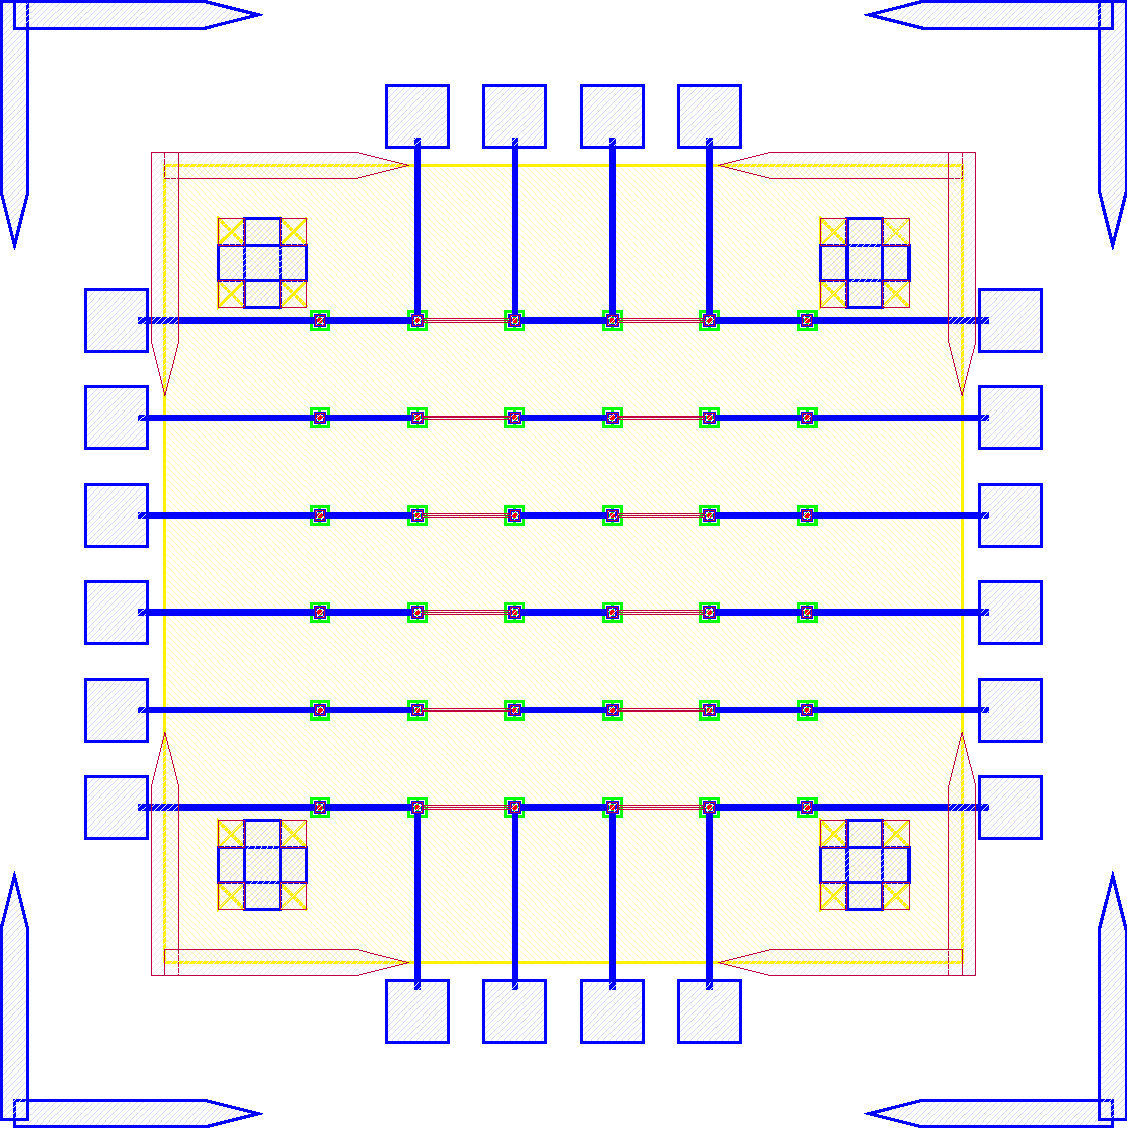
\includegraphics[width=0.4\textwidth]{Main/Ch2/DC_DieBTest_V5.GDStex_output.pdf}
    \caption{GDS file of bonded LED and BP. }
    \label{fig:ch3_gds_bp_led_anchors}
\end{figure}


\section{Characterization of Electrical Connection}

Going through the entire electroplating and diebonding process, I was able to begin the process of characterizing the electrical properties of the diebonds. As I was using the micromanipulator in E3-3177 there were certain limitations and intricacies to using the tool that were not relevant to the characterization, but I felt the need to mention.

\begin{itemize}
    \item The diebonded samples were significantly larger than the field of view of the microscope. This meant I had to translate the sample stage to move the test pads into view.
    \item Some probes suffered from significant static friction and high damping ratio which meant that translation of those probes faced significant lag when being used.
    \item One of the ocular lenses had a focal distance outside the z-axis range of the stage.
    \item The ocular lenses also faced significant vignetting.
    \item Some geared belt drives did not work.
\end{itemize}

While the previous issues did exist, there were no functional issues with the micromanipulator and the tool was absolutely functional for use in this situation.

\section{Connection Issues}
To complete the electrical characterization of the daisy-chain samples, the probes of the micromanipulator were attached to a Kiethley Source Measurement Unit (SMU). The SMU allows us to apply voltages and currents and measure voltages, currents, and resistances. Upon attempting to measure the resistance of the sample, at first an `overflow' or open-circuit was measured.

To overcome this at first a small voltage below $1 \V$ and was gradually increased up-to $20 \V$ until a current was measured. This procedure of applying a high voltage is likely similar to what is often seen in oxide breakdown of transistors \cite{oxide_breakdown} where an oxide layer is broken down and promotes the creation of a conductive material from the source to discharge point. However, it is still unclear as to why this surface oxide appears as indium should not have formed a surface oxide layer as according to \cite{indiumCorpSurfacePrep} an oxide layer of a maximum of $80-100 \unit{\angstrom}$ would form after $2-4\unit{\hour}$ this oxide layer should have been removed by the preceding plasma-cleaning step \cite{plasma_clean_oxide} and diebonding should have easily melted the indium forming a bond that would work.

Once connection issues were resolved the resistance over the pads were measured. While measuring, however, the resistances over the pads was constantly in flux at a rate of change of $\frac{1-4 \unit{\ohm}}{\unit{\minute}}$.

\section{Conformation to Theory}

The results of the measurements were as follows from table \ref{tab:daisychain_resistance_table}.

\begin{table}
    \centering
    \begin{subtable}[t]{0.3\textwidth}
        \centering
        \begin{tabular}{| l | l | c |}
            \hline
            Start & End & Resistance [$\Omega$] \\
            \hline
            \hline
            $v_{i_1}$ & $v_{o_{1,1}}$ & $64$ \\
            $v_{i_1}$ & $v_{o_{1,2}}$ & $44$ \\
            $v_{i_1}$ & $v_{o_{1,3}}$ & $69$ \\
            $v_{i_6}$ & $v_{o_{6,1}}$ & $54$ \\
            $v_{i_6}$ & $v_{o_{6,2}}$ & $65$ \\
            $v_{i_6}$ & $v_{o_{6,3}}$ & $56$ \\
            \hline
        \end{tabular}
        \caption{Sample 1.}
    \end{subtable}
    ~
    \begin{subtable}{0.3\textwidth}
        \centering
        \begin{tabular}[t]{| l | l | c |}
            \hline
            Start & End & Resistance [$\Omega$] \\
            \hline
            \hline
            $v_{i_1}$ & $v_{o_{1,5}}$ & $\infty$ \\
            $v_{i_2}$ & $v_{o_{2,5}}$ & $1,000,000$ \\
            \hline
        \end{tabular}
        \caption{Sample 2. Sample damaged after improper use of micromanipulator.}
    \end{subtable}
    ~
    \begin{subtable}[t]{0.3\textwidth}
        \centering
        \begin{tabular}{| l | l | c |}
            \hline
            Start & End & Resistance [$\Omega$] \\
            \hline
            \hline
            $v_{i_1}$ & $v_{o_{1,5}}$ & $90$ \\
            $v_{i_2}$ & $v_{o_{1,5}}$ & $95$ \\
            $v_{i_3}$ & $v_{o_{1,5}}$ & $85$ \\
            $v_{i_4}$ & $v_{o_{1,5}}$ & $80$ \\
            $v_{i_5}$ & $v_{o_{1,5}}$ & $90$ \\
            $v_{i_6}$ & $v_{o_{1,5}}$ & $71$ \\
            \hline
        \end{tabular}
        \caption{Sample 3.}
    \end{subtable}
    \caption{Daisy-chain resistance measurements of samples. Equivalent schematic figure \ref{fig:daisychain_circuits}.}
    \label{tab:daisychain_resistance_table}
\end{table}

Since the resistance of each section of the daisy-chain circuit can have some theoretical resistance calculated using a basic equation for resistance \ref{eq:resistance} where the resistance is given by some function of the resistivity, length and cross-sectional area of the wire. Similarly, using the equivalent schematic from figure \ref{fig:daisychain_circuits} we can try to characterize the resistance of the indium bonds.

\begin{figure}
    \centering
    \begin{subfigure}[b]{\textwidth}
        \centering
        \begin{circuitikz} \draw
            node[above]{$v_{i_1}$} (0,0)
            to[R=$R_{Au}$, o-] (2,0)
            to[R=$R_{In}$, -] (2,-2)
            to[R=$R_{Au}$, -] (4,-2)
            to[R=$R_{In}$, -] (4,0)
            to[R=$R_{Au}$, -] (6,0)
            to[R=$R_{In}$, -] (6,-2)
            to[R=$R_{Au}$, -] (8,-2)
            to[R=$R_{In}$, -] (8,0)
            to[R=$R_{Au}$, -o] (10,0)
            node[above]{$v_{o_{1,5}}$}
            ;
            % Draw pads
            \draw (2,0)
            to[R=$R_{Au}$, -o] (2, 2)
            node[above]{$v_{o_{1,1}}$};
            \draw (4,0)
            to[R=$R_{Au}$, -o] (4, 2)
            node[above]{$v_{o_{1,2}}$};
            \draw (6,0)
            to[R=$R_{Au}$, -o] (6, 2)
            node[above]{$v_{o_{1,3}}$};
            \draw (8,0)
            to[R=$R_{Au}$, -o] (8, 2)
            node[above]{$v_{o_{1,4}}$};
        \end{circuitikz}
        \caption{Representative circuit of top row.}
        \label{fig:daisychain_row1}
    \end{subfigure}
~
    \begin{subfigure}[b]{\textwidth}
        \centering
        \begin{circuitikz} \draw
            node[above]{$v_{i_j}$} (0,0)
            to[R=$R_{Au}$, o-] (2,0)
            to[R=$R_{In}$, -] (2,-2)
            to[R=$R_{Au}$, -] (4,-2)
            to[R=$R_{In}$, -] (4,0)
            to[R=$R_{Au}$, -] (6,0)
            to[R=$R_{In}$, -] (6,-2)
            to[R=$R_{Au}$, -] (8,-2)
            to[R=$R_{In}$, -] (8,0)
            to[R=$R_{Au}$, -o] (10,0)
            node[above]{$v_{o_{j,5}}$}
            ;
        \end{circuitikz}
        \caption{Representative circuit of middle 4 rows, $j \in \{2, 3, 4, 5\}$.}
        \label{fig:daisychain_row2345}
    \end{subfigure}
~
    \begin{subfigure}[b]{\textwidth}
        \centering

        \begin{circuitikz} \draw
            node[above]{$v_{i_6}$} (0,0)
            to[R=$R_{Au}$, o-] (2,0)
            to[R=$R_{In}$, -] (2,2)
            to[R=$R_{Au}$, -] (4,2)
            to[R=$R_{In}$, -] (4,0)
            to[R=$R_{Au}$, -] (6,0)
            to[R=$R_{In}$, -] (6,2)
            to[R=$R_{Au}$, -] (8,2)
            to[R=$R_{In}$, -] (8,0)
            to[R=$R_{Au}$, -o] (10,0)
            node[above]{$v_{o_{6,5}}$}
            ;
            % Draw pads
            \draw (2,0)
            to[R=$R_{Au}$, -o] (2, -2)
            node[below]{$v_{o_{6,1}}$};
            \draw (4,0)
            to[R=$R_{Au}$, -o] (4, -2)
            node[below]{$v_{o_{6,2}}$};
            \draw (6,0)
            to[R=$R_{Au}$, -o] (6, -2)
            node[below]{$v_{o_{6,3}}$};
            \draw (8,0)
            to[R=$R_{Au}$, -o] (8, -2)
            node[below]{$v_{o_{6,4}}$};
        \end{circuitikz}
        \caption{Representative circuit of bottom row.}
        \label{fig:daisychain_row6}
    \end{subfigure}
    \caption{Equivalent circuit diagrams of daisy-chain tests}
    \label{fig:daisychain_circuits}
\end{figure}


\begin{equation}
    \begin{split}
        R &\doteq \frac{\rho L}{A} \\
        R &\doteq \sum^n_{i=1} R_{\ch{Au}} + \sum^n_{i=1} R_{\ch{In}}
    \end{split}
    \label{eq:resistance}
\end{equation}

For the full row of the circuit in figure \ref{fig:daisychain_circuits} the total resistivity is given by equation \ref{eq:resist_top}.

\begin{equation}
    \begin{split}
        R_{Total}   &\doteq \frac{\rho_{\ch{Au}} 1500 \um}{200\nm \times 20\um} + R_{\ch{In}} \\
                    &+ \frac{\rho_{\ch{Au}} 500 \um}{200\nm \times 20\um} + R_{\ch{In}} \\
                    &+ \frac{\rho_{\ch{Au}} 500 \um}{200\nm \times 20\um} + R_{\ch{In}} \\
                    &+ \frac{\rho_{\ch{Au}} 500 \um}{200\nm \times 20\um} + R_{\ch{In}} \\
                    &+ \frac{\rho_{\ch{Au}} 1500 \um}{200\nm \times 20\um} \\
        R_{Total}   &= 4 R_{\ch{In}} + \frac{\rho_{\ch{Au}} (1500 + 500 + 500 + 500 + 1500) \um}{200\nm \times 20\um} \\
        R_{\ch{In}} &= \frac{\frac{\rho_{\ch{Au}} 4500 \um}{200\nm \times 20\um} - R}{4} \\
        R_{\ch{In}} &= \frac{R_{Total} - 25}{4}
    \end{split}
    \label{eq:resist_top}
\end{equation}
% Resistance calculation
% https://www.wolframalpha.com/input?i=%28resistivity+of+gold+*+4500+um%29%2F%28200um+*+20nm%29
Similar calculations to equation \ref{eq:resist_top} can be done for the other portions of the daisy-chain tests.

This results in the bond electrical resistance values in figure \ref{fig:histogram_resist}.

\begin{figure}
    \centering
    \begin{tikzpicture}
        \begin{axis}[
            xlabel=Indium bond electrical resistnace ($\Omega$),
            ylabel=Number of bonds with resistance,
            grid = both,
            % xmode=log,
            % ymode=log,
            minor tick num = 1,
            major grid style = {lightgray},
            minor grid style = {lightgray!25},
            % legend pos=north west
            ybar,
            ymin=0
        ]
        \addplot +[
            purple4,
            hist={
                bins=7,
                % data min=0.5,
                % data max=4
            }
        ] table [y index=0] {Main/Ch3/resistance.dat};
        \end{axis}
    \end{tikzpicture}
    \caption{Histogram of daisy-chain test calculations of the resistance of the indium bonds}
    \label{fig:histogram_resist}
\end{figure}

\section{Development of a Repeatable Process}

% Keeping process temperature low
\subsection{Minimizing Process temperature}
Since we were observing bonds that were failing and being difficult potentially due to the surface oxidation, it was suggested to minimize the process temperature after the electroplating, as such the HMDS application step which reaches a temperature of $160\dC$ was removed. The other warm process steps


\subsection{Improving cleanliness of process}

I acquired a 4-inch wafer to place the LED on while it was being picked up for diebonding. The wafer is also surface activated and placed in the plasma cleaner with the rest of the samples to ensure it is also relatively clean. The wafer when not being used is placed in the wafer carrier tray.
The wafer was added to ensure that the surface energy of the LED sample when face-down is not affected as compared to when face down on the diebonder surface.

Furthermore, the bonding head is regularly cleaned with IPA before being used to minimize likelihood of sticking to the diebonder head.
% Plasma clean
% Clean Wafer